\documentclass[spanish, 10pt,a4paper]{article}
\usepackage[spanish]{babel}
\usepackage[utf8]{inputenc}
\usepackage{textcomp}
\usepackage{hyperref}
\usepackage[pdftex]{graphicx}
\usepackage{epsfig}
\usepackage{amsmath}
\usepackage{hyperref}
\usepackage{amssymb}
\usepackage{color}
\usepackage{graphics}
\usepackage{clrscode3e}
\usepackage{amsthm}
\usepackage{caratula}
\usepackage{fancyhdr,lastpage}
\usepackage[paper=a4paper, left=0.8cm, right=0.8cm, bottom=1.4cm, top=1.4cm]{geometry}
\usepackage[table]{xcolor} % color en las matrices
\usepackage[font=small,labelfont=bf]{caption} % caption de las figuras en letra mas chica que el texto
\usepackage[ruled,vlined,linesnumbered]{algorithm2e}
\usepackage{listings}
\usepackage{float}
\usepackage{amsfonts}
\usepackage{upgreek}
\usepackage{anysize} 
\usepackage[utf8]{inputenc}
\usepackage{babel}
\usepackage{hyperref}
\usepackage[pdftex]{graphicx}
\usepackage{amsfonts}
\usepackage{amsmath}
\usepackage{colortbl}
\usepackage{pdfpages}
\usepackage{titlesec}
\usepackage[margin=1cm]{subcaption}


\color{black}

%%%PAGE LAYOUT%%%
\topmargin = -1.2cm
\voffset = 0cm
\hoffset = 0em
\textwidth = 48em
\textheight = 164 ex
\oddsidemargin = 0.5 em
\parindent = 1 em
\parskip = 3 pt
\footskip = 7ex
\headheight = 20pt
\pagestyle{fancy}
\lhead{Redes Neuronales - 2017 C1 - Trabajo Pr\'actico} % cambia la parte izquierda del encabezado
\renewcommand{\sectionmark}[1]{\markboth{#1}{}} % cambia la parte derecha del encabezado
\rfoot{\thepage}
\cfoot{}
\numberwithin{equation}{section} %sets equation numbers <chapter>.<section>.<subsection>.<index>

%Lo siguiente controla el ancho de las figuras (principalmente para el texto de los captions)
%\newcommand{\figurewidth}{.9\textwidth}
\newcommand{\figurewidth}{1\textwidth}

\newcommand{\tuple}[1]{\ensuremath{\left \langle #1 \right \rangle }}
\newcommand{\Ode}[1]{\small{$\mathcal{O}(#1)$}}
\newtheorem{teorema}{Teorema}[section]


%El siguiente paquete permite escribir la caratula facilmente
\hypersetup{
  pdftitle={ TLeng TP },
  colorlinks,
  citecolor=black,
  filecolor=black,
  linkcolor=black,
  urlcolor=black 
}

\materia{Redes Neuronales}

\titulo{Trabajo Práctico 1}

\subtitulo{Perceptrón Multicapa}

\grupo{Grupo X}

\integrante{Bonet, Felipe}{668/08}{fpbonet@gmail.com}
\integrante{Martínez, Federico}{XXX/XX}{fedomartinez@hotmail.com}
\integrante{Avendano, Demian}{XXX/XX}{demian.avendano@gmail.com}
 
\begin{document}
{ \oddsidemargin = 2em
	\headheight = -20pt
	\maketitle
}
	\tableofcontents
	\newpage
	
\section{Introducción}


\textit{En este documento se realizan las actividades propuestas en el TP 1, actividades relacionadas con la implementación de una red neuronal feedforward multicapa, con el fin de lograr predicciones sobre un set de datos, mientras se estudia su comportamiento durante el entrenamiento, en el contexto de un paradigma de aprendizaje supervizado.}

\subsection{Introducción al problema}
Las redes neuronales son modelos computacionales, en los que se intenta emular el funcionamiento fisiológico de un conjunto de neuronas biológicas, interconectadas, con el fin de lograr predicciones a partir de un conjunto de datos similares, presentados previamente. Para ello se modelan, en cada unidad de procesamiento, características que tienen que ver con las condiciones de propagación de señales electroquímicas. Estas condiciones se describen y modelan a partir de observaciones de sobre cómo es transmitida información entre una neurona y otra (o sobre si), y sobre como se encuentran interconectadas.

La suma de las interacciones entre estas unidades modeladas en una topología dada, genera propiedades emergentes que permiten  resolver cierto tipos de  problemas (caracterizados por el \textit{Teorema de la Aproximación Universal}). 
Para intentar resolver estos problemas utilizando una red neuronal, es necesario recurrir a diversas técnicas para el ajuste de las variables de la red, y en muchos casos se requiere un paso de preprocesamiento de los datos. 

Se implemento una red neuronal multicapa para la predicción de dos set de datos: el primer set, tiene que ver con el diagnóstico de cancer de mamas, los datos de entrada son valores reales, mientras que el dato de salida es la presencia o no de la enfermedad; el segundo set de datos tiene que ver con la eficiencia energética de la regulación de la temperatura de un edificio, los valores de entrada son tanto enteros como reales, existen dos valores de salida reales, que tienen que ver con la carga de calefacción y de refrigeración.  

\subsection{Entrega}
\subsection{Requerimientos}
\begin{itemize}
\item Intérprete python 2.7.
\item Librerías estandar, librería \textit{matplotlib} y \textit{numpy}.
\item Archivo CSV con uno de los dos formatos propuestos en el TP. 
\item Puede ser necesario instalar el paquete python-tk:
\textit{sudo apt-get install python-tk}
\end{itemize}

\subsection{Modo de uso y opciones}
Para usar este programa, se deben ejecutar el archivo \textbf{script.py}, el cual contiene todas las opciones de ejecución. Para ello, tipear por consola :

\texttt{\$python script.py N args}

donde \texttt{N} es el número de ejercicio y \texttt{args} son los argumentos optativos. Es obligatorio proveer el número de ejercicio, ya que se parsean los inputs de forma distinta. A su vez, cambian los métodos de cálculo de eficacia de la red.\\

Las opciones disponibles son:

\subsubsection{Opciones}

\textbf{-file}: Filepath del dataset que se desee utilizar para entrenar o predecir resultados. Si no se lo provee, por default el programa buscará el archivo $tp1_ej1_training.csv$ o $tp1_ej2_training.csv$ en la carpeta donde se esté ejecutando, dependiendo del número de ejercicio pasado anteriormente.

\textbf{-ep}: Cantidad de épocas por default, 500.

\textbf{-eta}: Tasa de aprendizaje, por default $\eta$ = 0.05

\textbf{-capas}: Capas ocultas de la red, cada número separado por una coma representa una capa y cada magnitud de la capa representa la cantaidad de neuronas de esa capa, por default = '10,10', o sea, dos capas de 10 neuronas cada una.

\textbf{-tr}:  Cantidad en \% del total de datos utilizado para entrenar a la red, por default = 70.

\textbf{-te}: Cantidad en \% del total de datos utilizado para testing, por default = 20

\textbf{-val}: Cantidad en \% del total de datos utilizados como validación, por default = 10

\textbf{-tambatch}: Tamaño del batch de aprendizaje a utilizar. Por default el valor es $1$, es decir entrenamiento estocástico.

\textbf{-mo}: Magnitud del momentum a utilizar. Default es 0.

\textbf{-fa}: Función de activación, puede ser \textit{tangente o logística}, por default es \textit{tangente}.

\textbf{-dp}: Distribución de inicialización de pesos a utilizar, puede ser \textit{normal} o \textit{uniforme}, por default se usa \textit{normal}.

\textbf{-rda}: Permite cargar una red entrenada desde un archivo con formato \textit{JSON}. Se debe proveer el filepath del archivo JSON. En caso de no proveer este parámetro, se generará una red nueva, entrenándola con el dataset seleccionado.

\textbf{-rha}: Permite almacenar una red entrenada a un archivo con \textit{JSON}. Se debe proveer el filepath destino del archivo JSON.

\textbf{-estop}: Utilizado para activar early stopping. El argumento es el treshold a considerar. Default = 0.

\textbf{-adap}: Define si se utiliza o no parámetros adaptativos. Valores = 0 o 1. Default = 0.

\subsection{Archivos}
Para la resolución del trabajo, fue necesario desarrollar en primer lugar un parser de los datos de entrada. El código de las funciones de parsing esta en \textbf{parser.py}.\\

El código propiamente de la red se encuentra en \textbf{perceptron.py}. Allí están todas las funciones de los procesos de inicialización, feedforward, backpropagation y otros asociados.\\

El parsing y definición de parámetros está en \textbf{parameters.py}. Las funciones encargadas de la normalización de los datos se encuentra en \textbf{normalizer.py}. Las funciones encargadas de codificar y decodificar redes entrenadas en formato json se hallan en \textbf{encoder.py}


\subsection{Otros scripts}

Se proveen a su vez los scripts utilizados para los experimentos, en caso de desear ejecutarlos. En la sección Resultados comentaremos donde se encuentra el código utilizado para cada uno.

	\newpage
	\section{Desarrollo}


	\newpage
	\section{Resultados}
En esta sección incluiremos los resultados de la experimentación que realizamos con el perceptrón desarrollado.\\
La idea general de los experimentos es intentar medir la influencia de alguna(s) variable(s) específicas sobre la performance
de la red. Para ello intentamos fijar todas las demás variables en valores óptimos y poner a prueba las que nos interesaban.\\

A medida que fuimos encontrando valores óptimos para las distintas variables, los fuimos utilizando para el resto de los experimentos subsiguientes.\\

En el primer experimento, intentamos determinar el mejor número de capas ocultas para utilizar en el ejercicio 1. A continuación, los resultados.

\subsection{Ejercicio 1}

\subsubsection{Variación del número de capas ocultas.}
La idea de este experimento es determinar la cantidad de capas ocultas óptimas para el ejercicio 1. Para ello fijamos las demás variables con esta configuración:

\begin{itemize}
\item Épocas: 250
\item ETA: 0.05
\item 10 neuronas por capa.
\item 70 \% del dataset como training, 20 \% training, 10\% validación.
\item Distribución de Pesos: Normal
\item Entrenamiento Estocástico
\item Sin Momentum
\item Sin Early Stopping
\end{itemize}

Esta configuración es arbitraria y está basada en pruebas informales que realizó el equipo antes de comenzar la experimentación formal. A medida que avanzaron los experimentos y fuimos descubriendo mejores valores, los fuimos actualizando para las siguientes pruebas.\\

El experimento fue desarrollado así: 
\begin{itemize}
\item Dividimos el dataset en datos de entrenamiento, validación y testing. Utilizamos la misma división para todas las ejecuciones.
\item Con la configuración mencionada, corrimos 8 rondas de cada número de capas ocultas utilizando: 1, 2, 3, 5 y 10 capas.
Es decir, primero se ejecutaron 8 veces el entrenamiento, validación y testing de una red con 1 capa. Luego repetimos con 2, con 3, etc.
\item Para cada cantidad de capas, promediamos los resultados de cada una de las 8 rondas. Con ello obtuvimos un error final (función de costo) de entrenamiento promedio , un error de validación promedio y una efectividad de testing promedio. Llamamos efectividad de testing a la cantidad de resultados del dataset de testing correctamente predichos.

\item El error final de cada ronda corresponde a la función de costo de dicha corrida dividido la cantidad de patrones procesados.
\end{itemize}

Observemos los resultados:\\

\begin{figure}[h]
  \begin{center}
  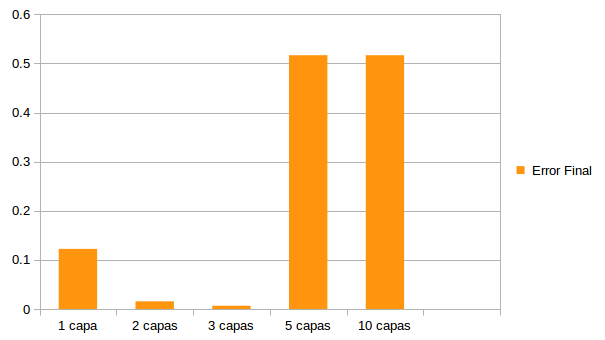
\includegraphics[scale=0.75]{graficos/fig1_cant_capas_error_final.png}
  \caption{Error final (función de costo) promedio para cada cantidad de neuronas utilizando el dataset de entrenamiento}
  \end{center}
\end{figure}

Podemos ver en la figura 1 que los mejores errores fueron obtenidos con 2 y 3 capas. Estos datos pertenecen al error final promediado, usando el dataset de entrenamiento.\\
Notamos también que con más de 3 capas ya los números se empiezan a distorsionar y perder mucha precisión.

Para el error final en los datos de validación, obtuvimos los siguientes resultados:\\

\begin{figure}[h]
  \begin{center}
  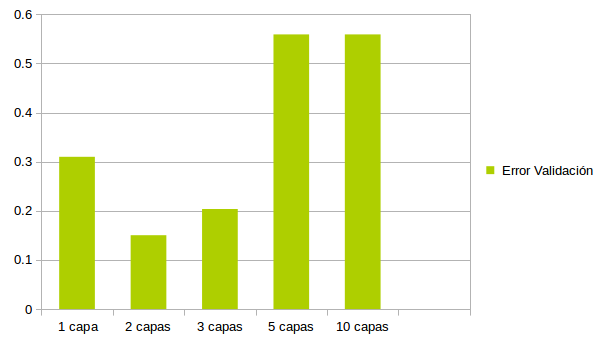
\includegraphics[scale=0.75]{graficos/fig2_cant_capas_error_valid.png}
  \caption{Error (función de costo) promedio para cada cantidad de neuronas utilizando el dataset de validación}
  \end{center}
\end{figure}


En la figura 2 podemos notar que el valor de error con el dataset de validación también 
genera mejores números con 2 y 3 capas. Especialmente se aprecia un mejor valor para la arquitectura de 2 capas.\\
Observamos nuevamente que los valores más altos no rinden igual de bien que los anteriores.

\begin{figure}[h]
  \begin{center}
  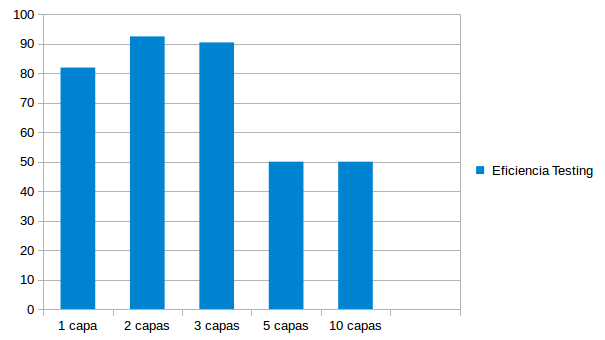
\includegraphics[scale=0.75]{graficos/fig3_cant_capas_testing.png}
  \caption{Tasa de predicciones correctas, en porcentaje, para el dataset de testing}
  \end{center}
\end{figure}

Para la efectividad en la predicción de los datos de testing, observamos en la figura 3 que la red de 1 capa generó aciertos cercanos al 82\%, mientras que las de 2 y 3 capas superan el 90\%, teniendo la de 2 capas un desempeño levemente mejor.\\
Nos sorprendíó ver que las redes de 5 y 10 capas lograron una muy baja eficiencia, cercana al 50\%.\\

Teniendo en cuenta los resultados presentados en estas pruebas, nos decidimos por una arquitectura de 2 capas ocultas. Aunque se obtuvieron resultados casi igual de buenos con arquitectura de 3 capas, \textbf{la de 2 capas presenta mejor velocidad de ejecución y resultados levemente mejores}.\\

\newpage

\subsubsection{Variación del número de neuronas ocultas.}

Una vez obtenido el número óptimo de capas ocultas, quisimos determinar cual era la cantidad de nueronas que debía contener
cada una de estas capas. Para simplificar el problema, decidimos que todas las capas tuvieran la misma cantidad de neuronas.\\
De esta forma, elegimos las siguientes medidas: 2 capas de 2, 5, 7, 10, 15 y 20 neuronas. Estas medidas fueron elegidas para intentar representar una cantidad baja de neuronas como 2,5,7 y otras más altas, por arriba de 10. No consideramos cantidades mayores de neuronas ya que los resultados no mejoran ostensiblemente pasando las 20 neuronas, teniendo en cuenta la relativa
sencillez del ejercicio en cuestión. Además, arquitecturas con más de 20 neuronas por capa afectan notablemente la velocidad de ejecución de la red, relentizando las pruebas y haciéndolas engorrosas e innecesarias.\\

De forma similar al experimento anterior, esta prueba consistió en procesar el dataset completo 8 veces con cada cantidad de neuronas distintas, promediar los errores finales de entrenamiento y de validación junto con la eficiencia obtenida en los datos de testing.\\
Para el error final, obtuvimos los siguientes resultados:\\

\begin{figure}[h]
  \begin{center}
  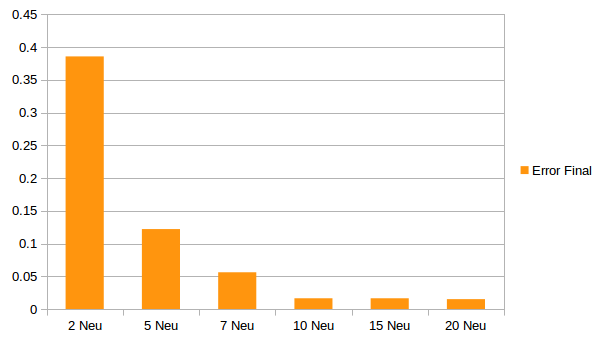
\includegraphics[scale=0.75]{graficos/fig4_cant_neuro_error_final.png}
  \caption{Error final (función de costo) promedio para cada cantidad de neuronas utilizando el dataset de entrenamiento}
  \end{center}
\end{figure}

En la figura 4 se puede observar que el valor de la función de costo decrece a medida que la cantidad
de neuronas crece. Este efecto se vuelve mucho menos notable a partir de las 10 neuronas por capa.\\

Para el error final en los datos de validación, obtuvimos los siguientes resultados:\\

\begin{figure}[h]
  \begin{center}
  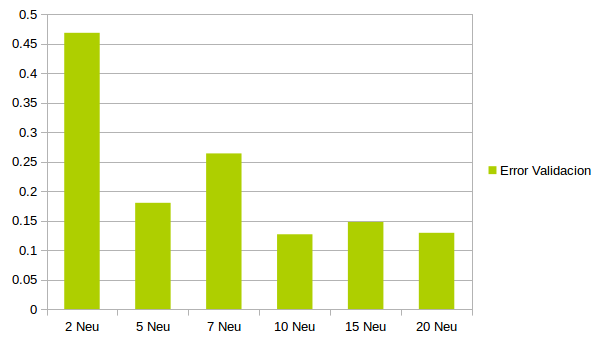
\includegraphics[scale=0.75]{graficos/fig5_cant_neuro_error_valid.png}
  \caption{Error (función de costo) promedio para cada cantidad de neuronas utilizando el dataset de validación}
  \end{center}
\end{figure}

En la figura 5 podemos notar que el valor de error con el dataset de validación también decrece a medida que sube la cantidad
de neuronas, aunque no de forma uniforme. Podemos apreciar que a partir de las 10 neuronas, el error se mantiene por debajo de 0.15.\\

Para la efectividad en la predicción de los datos de testing, observamos:\\

\begin{figure}[h]
  \begin{center}
  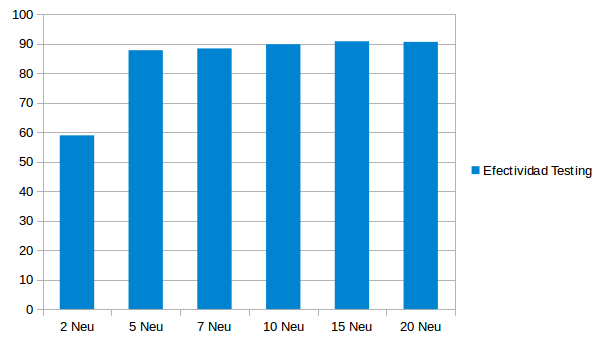
\includegraphics[scale=0.75]{graficos/fig6_cant_neuro_testing.png}
  \caption{Tasa de predicciones correctas, en porcentaje, para el dataset de testing}
  \end{center}
\end{figure}

Nuevamente podemos apreciar en la figura 6, que a medida que crece la cantidad de neuronas, crece la cantidad de aciertos sobre el conjunto de datos de test. Sin embargo, los resultados se comienzan a estancar a partir de las 10 neuronas en valores cercanos al 90 \% de aciertos.\\

Observando los resultados obtenidos en las pruebas, decidimos que la mejor configuración es con 10 neuronas por capa. Esta decisión se justifica teniendo en cuenta que los resultados no mejoran demasiado pasando de 10 y si empeora notablemente la velocidad de la red.\\
Por ende, \textbf{en vistas a los buenos resultados obtenidos con 10 neuronas y no obteniendo mejoras sustanciales con cantidades mayores}, nos quedaremos con este valor.

\subsubsection{Performance de la red, con entrenamiento sin momentum y con momentum.}

El momentum es una memoria o inercia que nos permite que los cambios en el vector de pesos $w$ sean suaves ya que incluyen información sobre el cambio de peso anterior. 
En el proceso de backpropagation de la red, cuando actualizamos los pesos, utilizaremos el momentum de la siguiente manera:
\\
\\
$\Delta w_{ij}^{m} = \eta \delta_{i}^{m}V_{j}^{m} + \alpha \Delta w_{pq}^{m-1}$
\\

Para este experimento, mantenemos la configuración que veniamos utilizando en experimentos anteriores con 2 capas de 10 neuronas. Probaremos el comportamiento de la red 
variando el momentum desde $0$ (o sin momentum) hasta un valor de momentum de \textbf{0.9}. No utilizaremos valores mayores de \textbf{0.9} ya que significaría que el peso anterior que 
tenía el eje se estaría acumulando con el nuevo peso en su completitud, lo cual nos parece una exageración en este caso. Dado que en posteriores experimentos realizaremos
pruebas variando el momentum y el learning rate en conjunto, para este experimento, mantendremos el learning rate de \textbf{0.05}.

\begin{figure}[!htbp]
\centering
\begin{subfigure}{.5\textwidth}
  \centering
  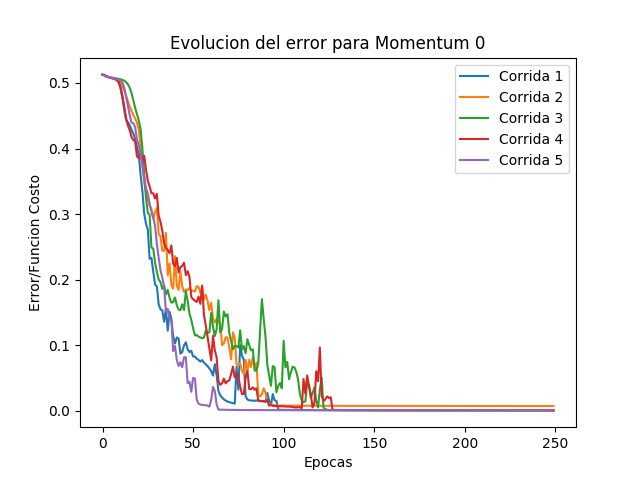
\includegraphics[width=1\linewidth]{graficos/momentum_0.png}
  \caption{Evolución del error de entrenamiento para momentum 0 (sin momentum)}
  \label{fig:sub1}
\end{subfigure}%
\begin{subfigure}{.5\textwidth}
  \centering
  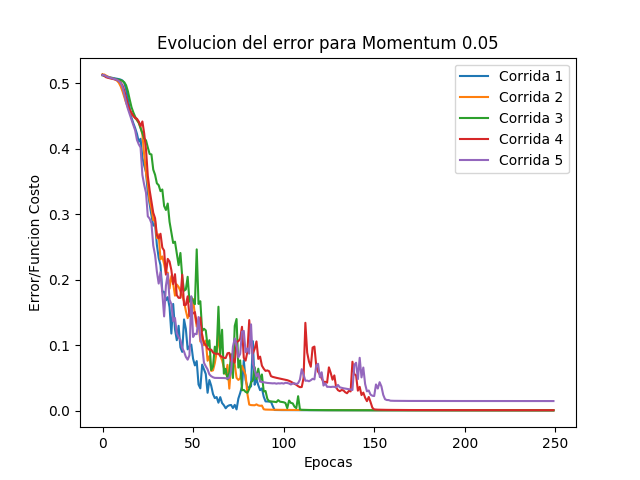
\includegraphics[width=1\linewidth]{graficos/momentum_0_05.png}
  \caption{Evolución del error de entrenamiento para momentum 0.05}
  \label{fig:sub2}
\end{subfigure}
\end{figure}

A partir de los resultados podemos intuir que manteniendo el learning rate elegido, no usar momentum o usar momentum \textbf{0.05 o 0.5} da los mejores resultados. Claramente
usar \textbf{0.9} es casi como al nuevo peso de cada eje sumarle el peso anterior, por eso la oscilación tan pronunciada. Sin embargo, y para llegar a una conclusión del mejor 
valor de momentum, analizemos los resultados de la evolución del error para nuestro conjunto de validación:

\begin{figure}[!htbp]
\centering
\begin{subfigure}{.5\textwidth}
  \centering
  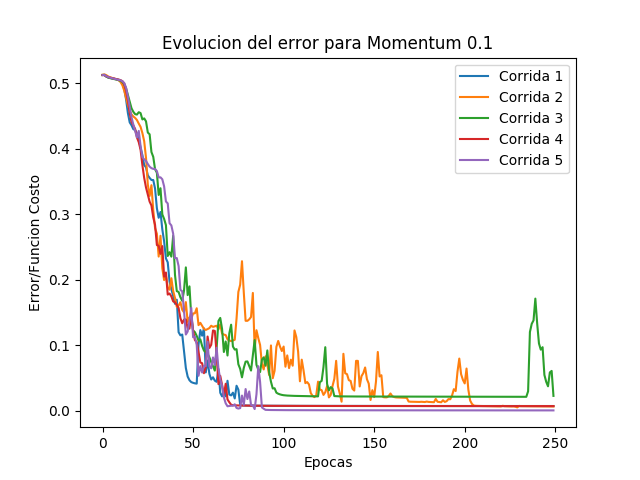
\includegraphics[width=1\linewidth]{graficos/momentum_0_1.png}
  \caption{Evolución del error de entrenamiento para momentum 0.1}
  \label{fig:sub1}
\end{subfigure}%
\begin{subfigure}{.5\textwidth}
  \centering
  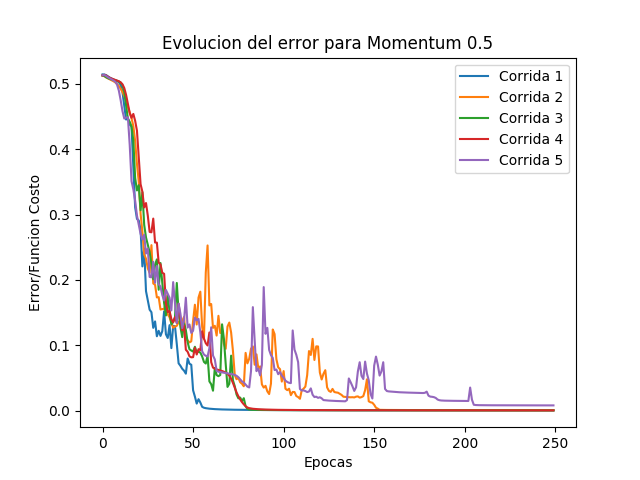
\includegraphics[width=1\linewidth]{graficos/momentum_0_5.png}
  \caption{Evolución del error de entrenamiento para momentum 0.5}
  \label{fig:sub2}
\end{subfigure}
\end{figure}

\begin{figure}[!htbp]
\centering
\begin{subfigure}{.5\textwidth}
  \centering
  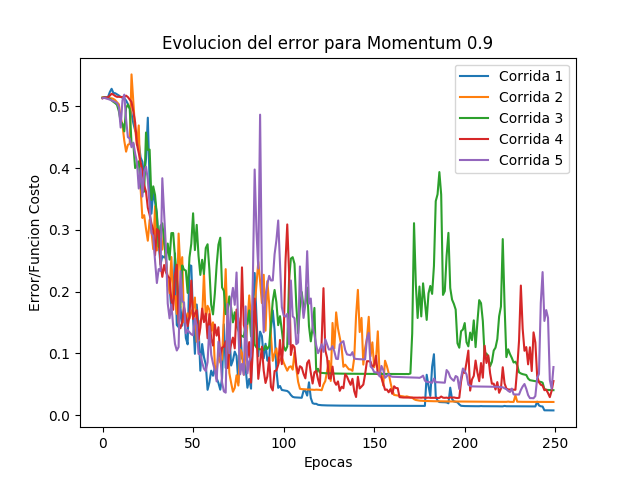
\includegraphics[width=1\linewidth]{graficos/momentum_0_9.png}
  \caption{Evolución del error de entrenamiento para momentum 0.9}
  \label{fig:sub1}
\end{subfigure}%
\begin{subfigure}{.5\textwidth}
  \centering
  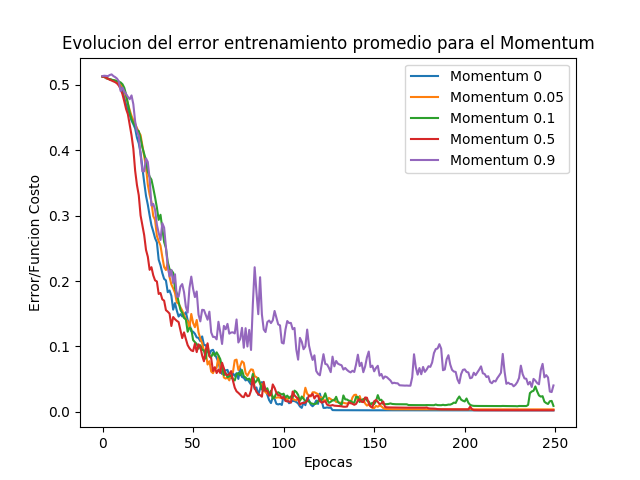
\includegraphics[width=1\linewidth]{graficos/momentum_promedios_entrenamiento.png}
  \caption{Evolución del error de entrenamiento promedio para todos los valores de momentum}
  \label{fig:sub2}
\end{subfigure}
\end{figure}

\begin{figure}[!htbp]
  \begin{center}
  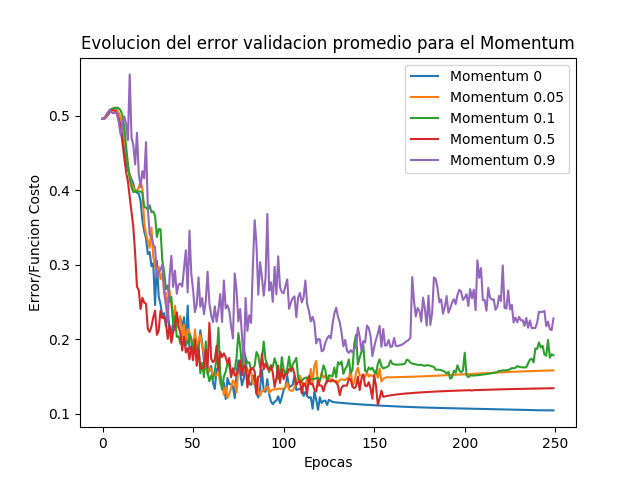
\includegraphics[scale=0.80]{graficos/momentum_promedios_validacion.png}
  \caption{Evolución del error de validación promedio para todos los valores de momentum}
  \end{center}
\end{figure}

Teniendo en cuenta ahora también nuestro error de validación final para todas las corridas y valores de momentum, podemos concluir entonces que manteniendo nuestro learning
rate fijo en \textbf{0.05}, lo mejor es no usar momentum.

\subsubsection{Performance de la red, con entrenamiento sin y con parámetros adaptativos.}

Utilizar parámetros adaptativos, como variar el learning rate, nos permiten volver a un estado anterior de la red y corregir el learning rate que usamos en 
ese momento para que esta vez nos de un mejor resultado. Para nuestra configuración adaptativa, si el error crece continuamente reducimos el learning a la mitad, 
mientras que si el error va en bajada, aumentamos el learning rate en un $10\%$. Manteniendo los parámetros de configuración que venimos utilizando, hicimos experimentos
sobre entrenamientos estocásticos, batch y mini batch. 

A partir de los resultados de entrenamiento estocástico, podemos observar que usar parámetros adaptativos no solo no ayuda al aprendizaje de la red, sino que
además lo perjudica en gran magnitud. Esto puede deberse principalmente a que la red esta continuamente ajustando sus pesos en cada entrada del dataset para
poder con el learning rate actual, mejorar la precisión y reducir el error. Si cambiamos el learning rate los pesos que ajustamos en cada paso dejan de tener
sentido y el entrenamiento termina dando malos resultados.

\begin{figure}[!htbp]
\centering
\begin{subfigure}{.5\textwidth}
  \centering
  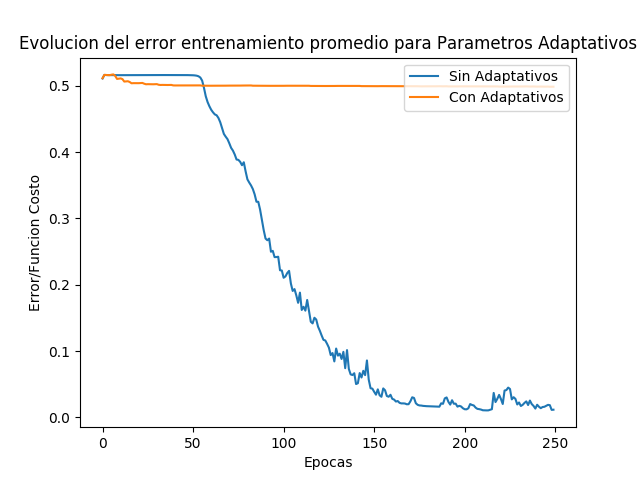
\includegraphics[width=1\linewidth]{graficos/adaptativos_promedios_entrenamiento.png}
  \caption{Comparación del error en el conjunto de entrenamiento para estocástico (250 épocas)}
  \label{fig:sub1}
\end{subfigure}%
\begin{subfigure}{.5\textwidth}
  \centering
  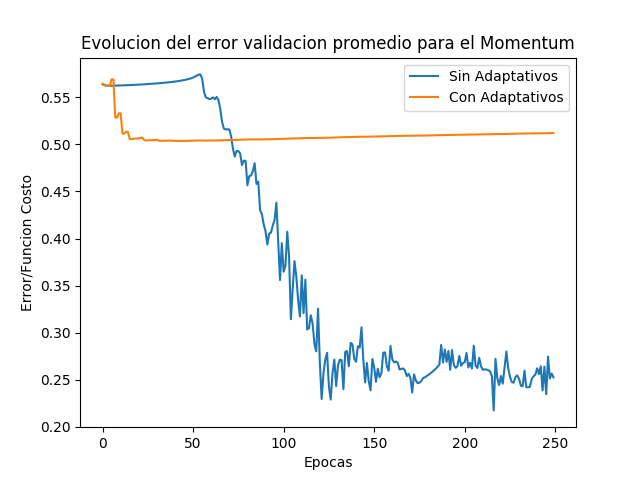
\includegraphics[width=1\linewidth]{graficos/adaptativos_promedios_validacion.png}
  \caption{Comparación del error en el conjunto de validación para estocástico (250 épocas)}
  \label{fig:sub2}
\end{subfigure}
\end{figure}

Con respecto a batch, nos dimos cuenta que los parámetros adaptativos permiten que se obtengan muy buenos resultados. Incluso se puede ver que el error de 
validación llega a ser menor que en el entrenamiento estocástico. Sin embargo, tuvimos que utilizar el doble de épocas para conseguir los mismos. 

\begin{figure}[!htbp]
\centering
\begin{subfigure}{.5\textwidth}
  \centering
  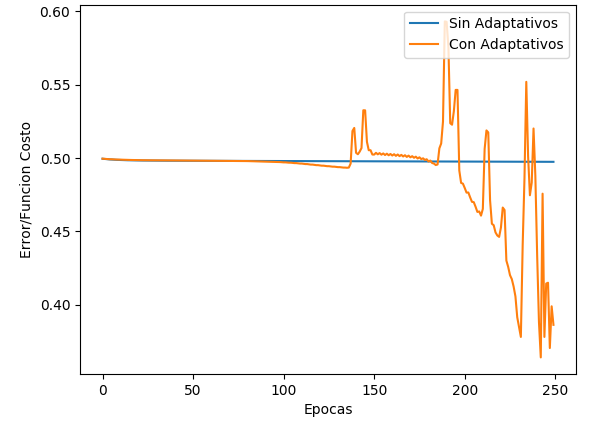
\includegraphics[width=1\linewidth]{graficos/adaptativos_promedios_entrenamiento_batch_05.png}
  \caption{Comparación del error en el conjunto de entrenamiento para batch (250 épocas)}
  \label{fig:sub1}
\end{subfigure}%
\begin{subfigure}{.5\textwidth}
  \centering
  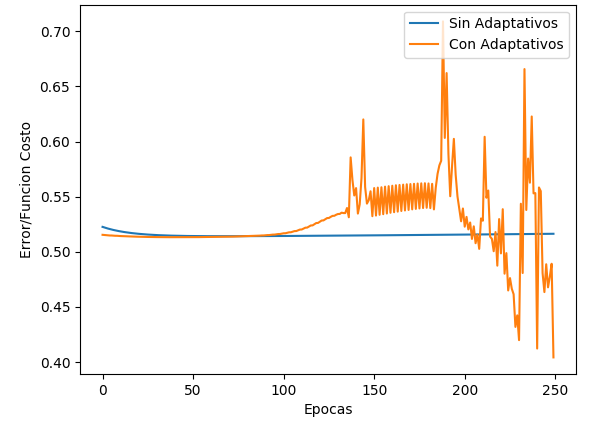
\includegraphics[width=1\linewidth]{graficos/adaptativos_promedios_validacion_batch_05.png}
  \caption{Comparación del error en el conjunto de validación para batch (250 épocas)}
  \label{fig:sub2}
\end{subfigure}
\end{figure}

\begin{figure}[!htbp]
\centering
\begin{subfigure}{.5\textwidth}
  \centering
  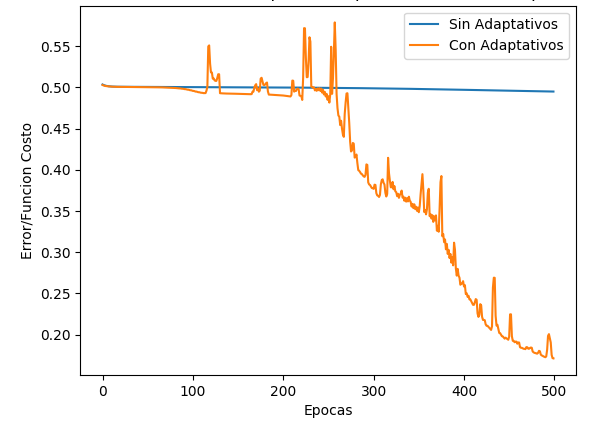
\includegraphics[width=1\linewidth]{graficos/adaptativos_promedios_entrenamiento_batch_500ep.png}
  \caption{Comparación del error en el conjunto de entrenamiento para batch (500 épocas)}
  \label{fig:sub1}
\end{subfigure}%
\begin{subfigure}{.5\textwidth}
  \centering
  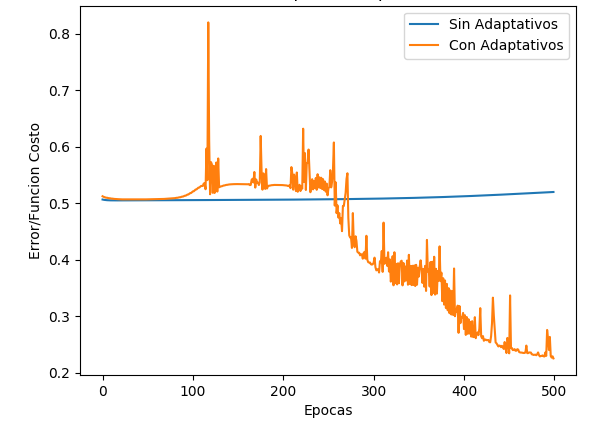
\includegraphics[width=1\linewidth]{graficos/adaptativos_promedios_validacion_batch_500ep.png}
  \caption{Comparación del error en el conjunto de validación para batch (500 épocas)}
  \label{fig:sub2}
\end{subfigure}
\end{figure}

Para el entrenamiento mini batch, confirma la idea de que el learning rate adaptativo es útil solo en batch y no para estocástico. Realizamos un par de
pruebas y vimos que mientras más cerca de 1 (estocástico) estuviese el tamaño del batch, peor resultados da el adaptivo, mientras que si más cerca está del
tamaño total del dataset de entrenamiento, mejor funciona el learning rate adaptativo. 

\begin{figure}[!htbp]
\centering
\begin{subfigure}{.5\textwidth}
  \centering
  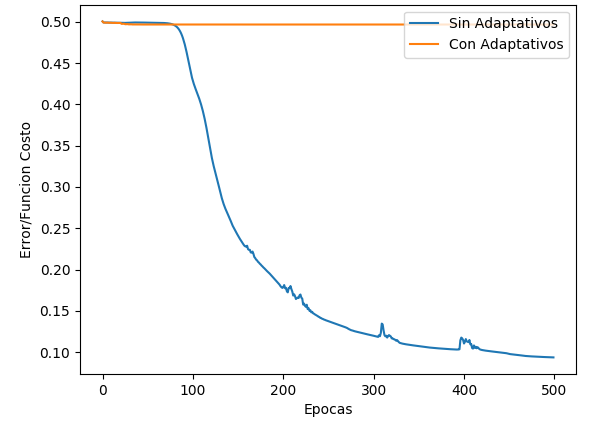
\includegraphics[width=1\linewidth]{graficos/adaptativos_promedios_entrenamiento_batch.png}
  \caption{Comparación del error en el conjunto de entrenamiento para mini batch de 10, cercano a ser estocástico (500 épocas)}
  \label{fig:sub1}
\end{subfigure}%
\begin{subfigure}{.5\textwidth}
  \centering
  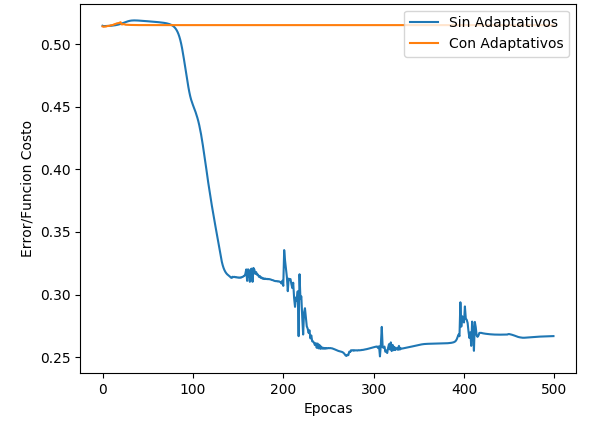
\includegraphics[width=1\linewidth]{graficos/adaptativos_promedios_validacion_batch.png}
  \caption{Comparación del error en el conjunto de validación para batch de 10, cercano a ser estocástico (500 épocas)}
  \label{fig:sub2}
\end{subfigure}
\end{figure}

Nuestra conclusión para este experimento es que si bien se llegan a alcanzar buenos resultados con el entrenamiento batch, es necesario utilizar el doble de épocas
lo cual hace que tarde mucho más el entrenamiento. Online learning en la mitad de las épocas y sin learning rate adaptativo obtiene resultados similares.

\subsubsection{Performance de la red, variando simultáneamente el factor de aprendizaje $\mu$, y el parámetro $\alpha$ del momentum.}

Para este experimento, utilizamos un conjunto de diferentes valores de momentums para diferentes valores del learning rate de manera de poder encontrar
donde se comportaba de mejor manera la red. El conjunto de valores de momentums es \textbf{0, 0.05, 0.1, 0.5 y 0.9}, los cuales se probaron con los valores
de learning rate \textbf{0.1, 0.05, 0.01, 0.005, 0.001}.

\begin{figure}[!htbp]
\centering
\begin{subfigure}{.5\textwidth}
  \centering
  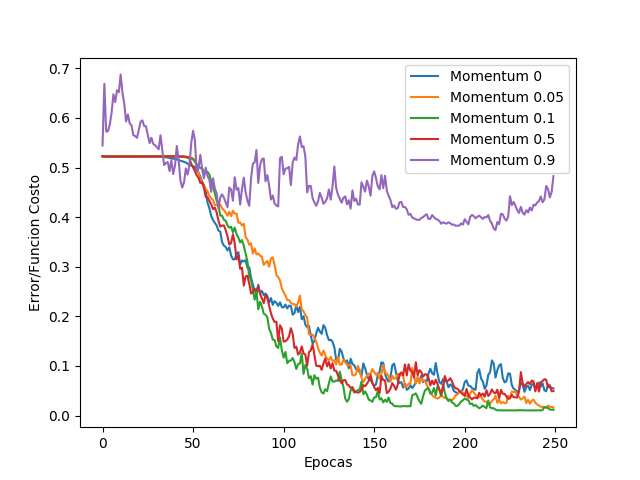
\includegraphics[width=1\linewidth]{graficos/eta_x_momentum_promedios_entrenamiento_0.png}
  \caption{Evolución del error de entrenamiento con momentum variable y learning rate fijo 0.1}
  \label{fig:sub1}
\end{subfigure}%
\begin{subfigure}{.5\textwidth}
  \centering
  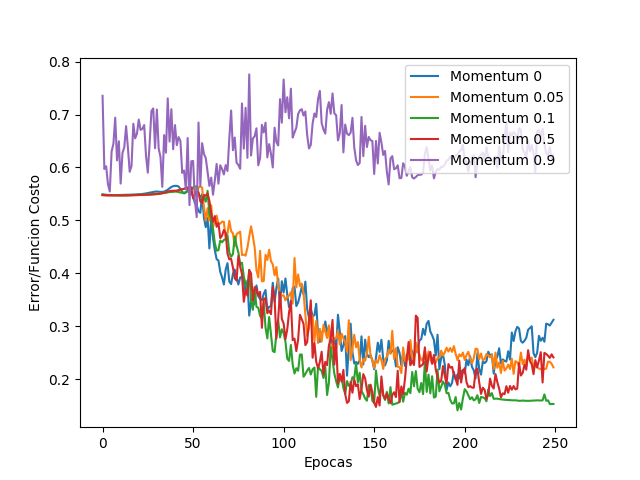
\includegraphics[width=1\linewidth]{graficos/eta_x_momentum_promedios_validacion_0.png}
  \caption{Evolución del error de validación con momentum variable y learning rate fijo 0.1}
  \label{fig:sub2}
\end{subfigure}
\end{figure}

\begin{figure}[!htbp]
\centering
\begin{subfigure}{.5\textwidth}
  \centering
  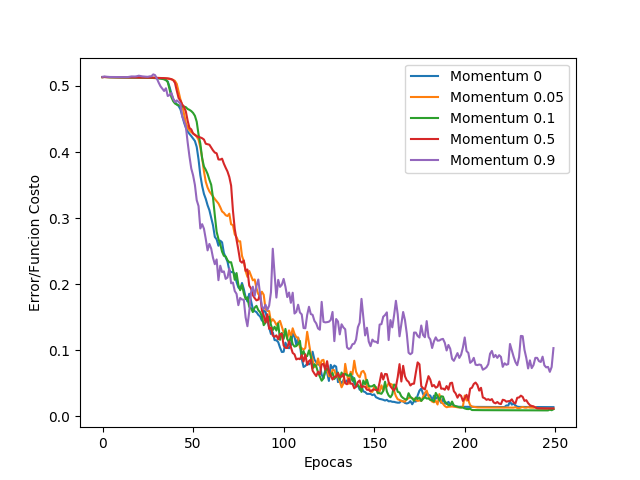
\includegraphics[width=1\linewidth]{graficos/eta_x_momentum_promedios_entrenamiento_1.png}
  \caption{Evolución del error de entrenamiento con momentum variable y learning rate fijo 0.05}
  \label{fig:sub1}
\end{subfigure}%
\begin{subfigure}{.5\textwidth}
  \centering
  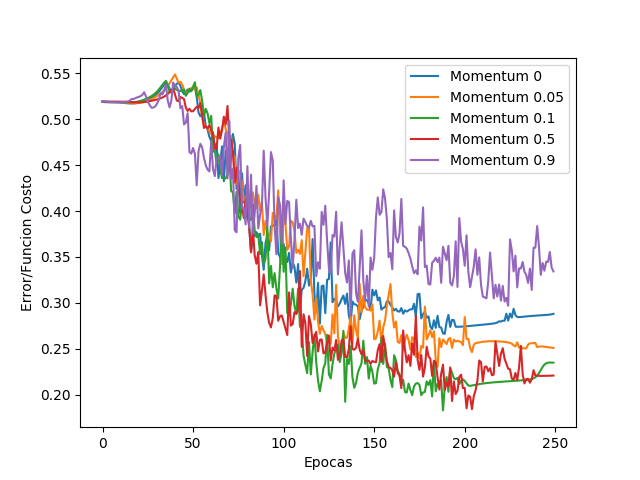
\includegraphics[width=1\linewidth]{graficos/eta_x_momentum_promedios_validacion_1.png}
  \caption{Evolución del error de validación con momentum variable y learning rate fijo 0.05}
  \label{fig:sub2}
\end{subfigure}
\end{figure}

\begin{figure}[!htbp]
\centering
\begin{subfigure}{.5\textwidth}
  \centering
  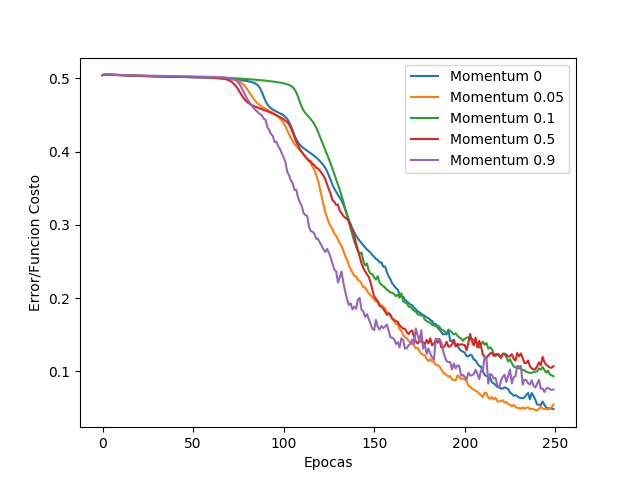
\includegraphics[width=1\linewidth]{graficos/eta_x_momentum_promedios_entrenamiento_2.png}
  \caption{Evolución del error de entrenamiento con momentum variable y learning rate fijo 0.01}
  \label{fig:sub1}
\end{subfigure}%
\begin{subfigure}{.5\textwidth}
  \centering
  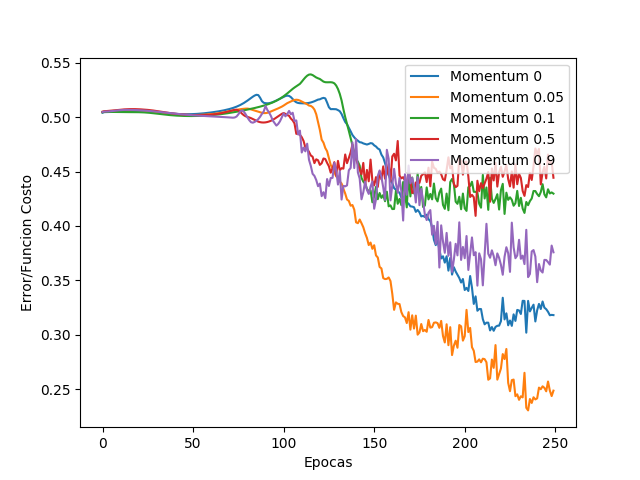
\includegraphics[width=1\linewidth]{graficos/eta_x_momentum_promedios_validacion_2.png}
  \caption{Evolución del error de validación con momentum variable y learning rate fijo 0.01}
  \label{fig:sub2}
\end{subfigure}
\end{figure}

\begin{figure}[!htbp]
\centering
\begin{subfigure}{.5\textwidth}
  \centering
  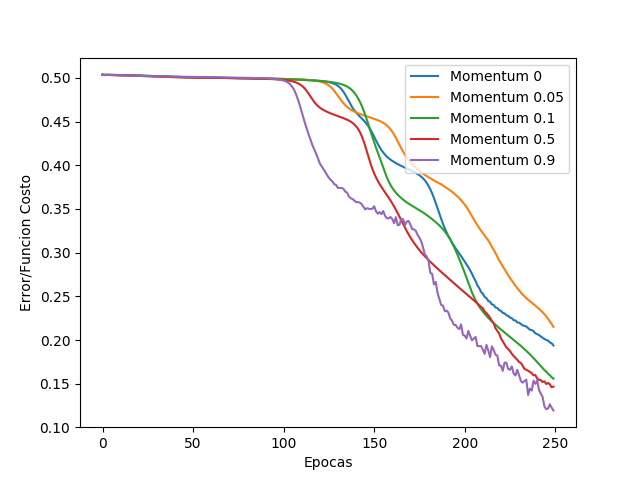
\includegraphics[width=1\linewidth]{graficos/eta_x_momentum_promedios_entrenamiento_3.png}
  \caption{Evolución del error de entrenamiento con momentum variable y learning rate fijo 0.005}
  \label{fig:sub1}
\end{subfigure}%
\begin{subfigure}{.5\textwidth}
  \centering
  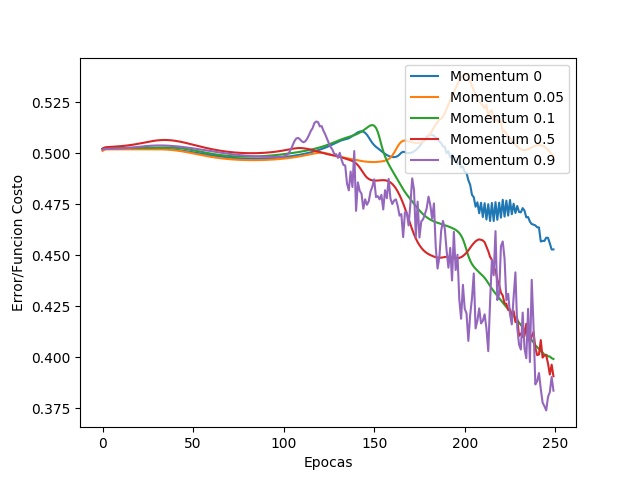
\includegraphics[width=1\linewidth]{graficos/eta_x_momentum_promedios_validacion_3.png}
  \caption{Evolución del error de validación con momentum variable y learning rate fijo 0.005}
  \label{fig:sub2}
\end{subfigure}
\end{figure}

\begin{figure}[!htbp]
\centering
\begin{subfigure}{.5\textwidth}
  \centering
  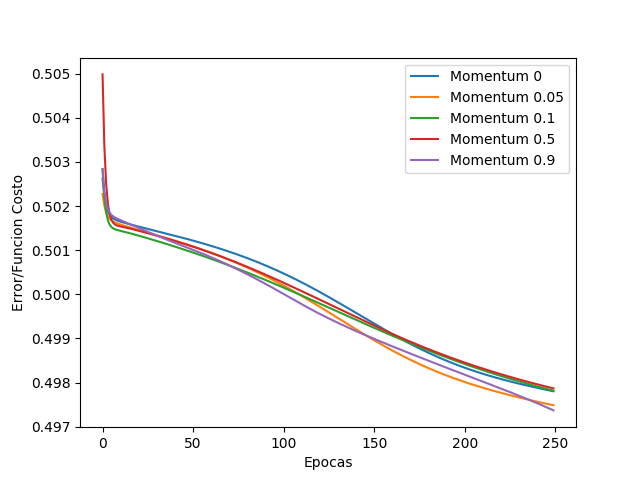
\includegraphics[width=1\linewidth]{graficos/eta_x_momentum_promedios_entrenamiento_4.png}
  \caption{Evolución del error de entrenamiento con momentum variable y learning rate fijo 0.001}
  \label{fig:sub1}
\end{subfigure}%
\begin{subfigure}{.5\textwidth}
  \centering
  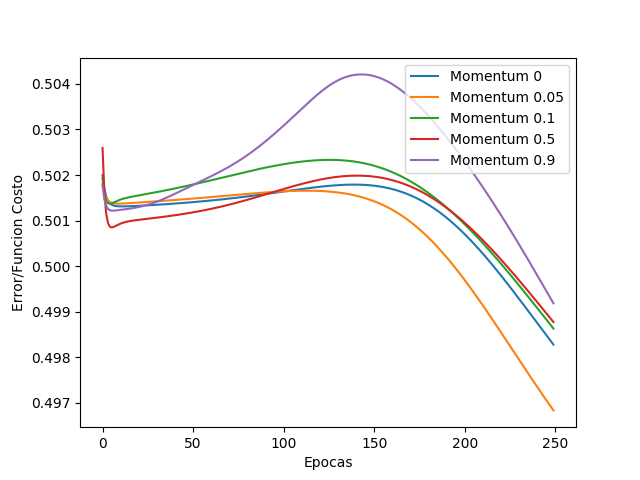
\includegraphics[width=1\linewidth]{graficos/eta_x_momentum_promedios_validacion_4.png}
  \caption{Evolución del error de validación con momentum variable y learning rate fijo 0.001}
  \label{fig:sub2}
\end{subfigure}
\end{figure}

A partir de los resultados podemos apreciar que los valores más bajos de error en entrenamiento y, aún más importante, en validación, se obtuvieron con
learning rate \textbf{0.1 y 0.05}. Es por eso que, siendo que cercanos a estos valores están nuestros mejores resultados, hicimos unas pruebas extras sobre
valores cercanos a los mismos. Esto es, probamos también con \textbf{0.08, 0.15 y 0.2} para intentar encontrar el mejor valor para nuestro learning rate en
entrenamiento estocástico.

\begin{figure}[!htbp]
\centering
\begin{subfigure}{.5\textwidth}
  \centering
  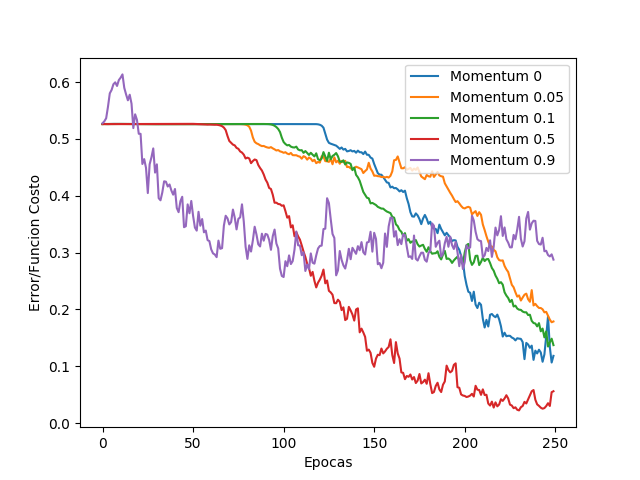
\includegraphics[width=1\linewidth]{graficos/eta_x_momentum_promedios_entrenamiento_0_08.png}
  \caption{Evolución del error de entrenamiento con momentum variable y learning rate fijo 0.08}
  \label{fig:sub1}
\end{subfigure}%
\begin{subfigure}{.5\textwidth}
  \centering
  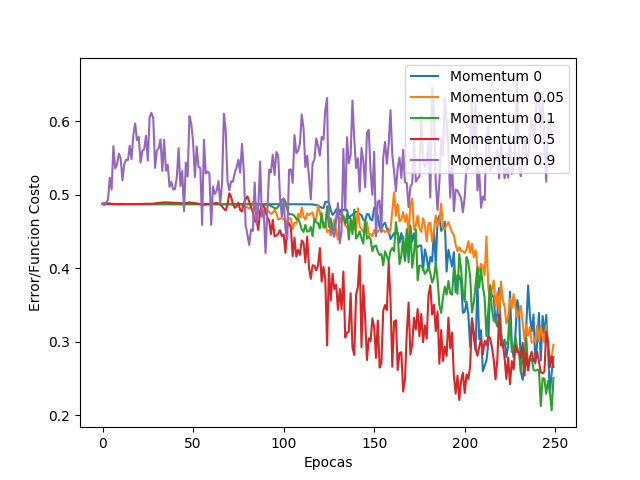
\includegraphics[width=1\linewidth]{graficos/eta_x_momentum_promedios_validacion_0_08.png}
  \caption{Evolución del error de validación con momentum variable y learning rate fijo 0.08}
  \label{fig:sub2}
\end{subfigure}
\end{figure}

\begin{figure}[!htbp]
\centering
\begin{subfigure}{.5\textwidth}
  \centering
  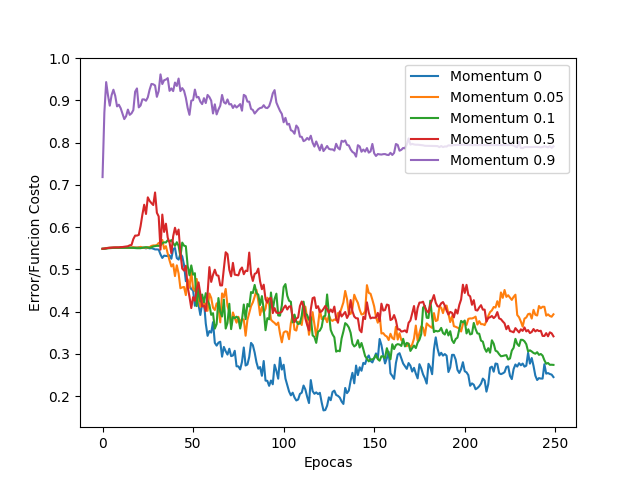
\includegraphics[width=1\linewidth]{graficos/eta_x_momentum_promedios_entrenamiento_0_15.png}
  \caption{Evolución del error de entrenamiento con momentum variable y learning rate fijo 0.15}
  \label{fig:sub1}
\end{subfigure}%
\begin{subfigure}{.5\textwidth}
  \centering
  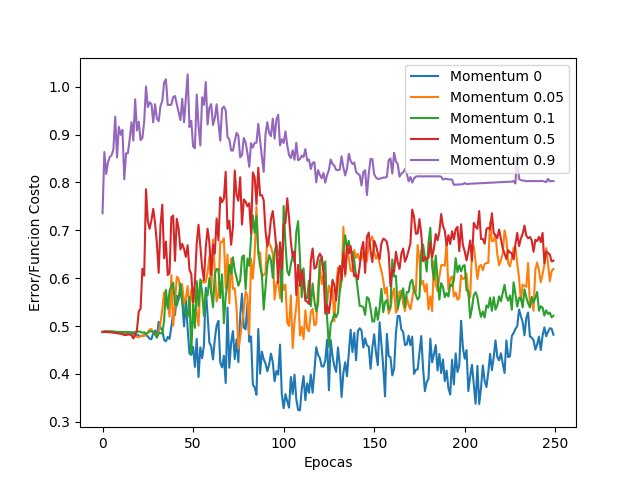
\includegraphics[width=1\linewidth]{graficos/eta_x_momentum_promedios_validacion_0_15.png}
  \caption{Evolución del error de validación con momentum variable y learning rate fijo 0.15}
  \label{fig:sub2}
\end{subfigure}
\end{figure}

\begin{figure}[!htbp]
\centering
\begin{subfigure}{.5\textwidth}
  \centering
  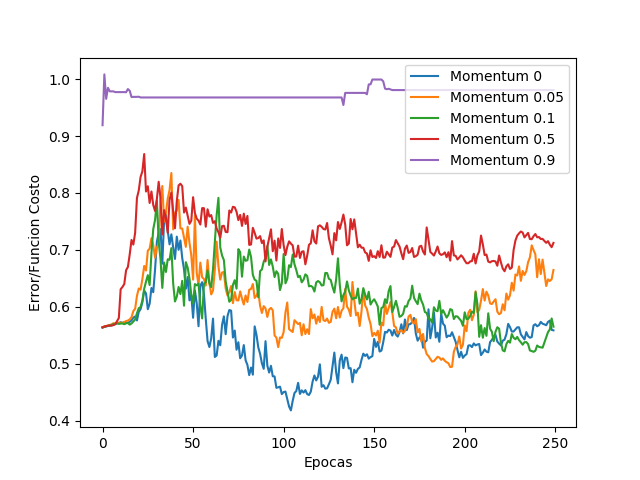
\includegraphics[width=1\linewidth]{graficos/eta_x_momentum_promedios_entrenamiento_0_2.png}
  \caption{Evolución del error de entrenamiento con momentum variable y learning rate fijo 0.2}
  \label{fig:sub1}
\end{subfigure}%
\begin{subfigure}{.5\textwidth}
  \centering
  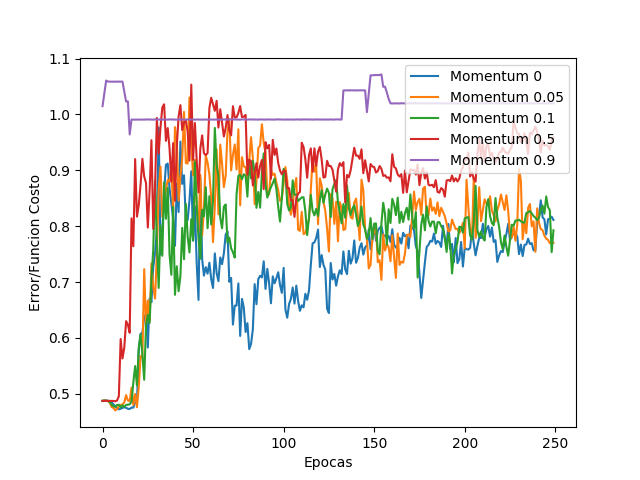
\includegraphics[width=1\linewidth]{graficos/eta_x_momentum_promedios_validacion_0_2.png}
  \caption{Evolución del error de validación con momentum variable y learning rate fijo 0.2}
  \label{fig:sub2}
\end{subfigure}
\end{figure}

Como se puede observar, los mejores resultados siguen siendo usando un learning rate de \textbf{0.1 y de 0.05}. Más interesante todavía es que en 
anteriores experimentos con el momentum y un learning rate de \textbf{0.05} habíamos visto que el momentum en \textbf{0} era la mejor opción. Sin embargo,
 en estos nuevos resultados se puede ver que usar momentum \textbf{0.1} es mejor que \textbf{0} tanto para el learning rate de \textbf{0.1 y de 0.05}. 
 Esto puede deberse a como se armaron los conjuntos de entrenamiento y validación, y para confirmarlo, volveremos a correr las pruebas para \textbf{0.1 y de 0.05}
 y compararlas.

\begin{figure}[!htbp]
\centering
\begin{subfigure}{.5\textwidth}
  \centering
  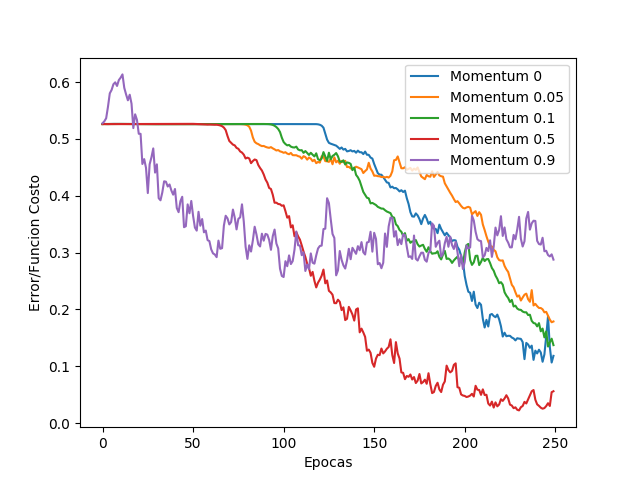
\includegraphics[width=1\linewidth]{graficos/eta_x_momentum_promedios_entrenamiento__0.png}
  \caption{Evolución del error de entrenamiento con momentum variable y learning rate fijo 0.05 (segunda vuelta)}
  \label{fig:sub1}
\end{subfigure}%
\begin{subfigure}{.5\textwidth}
  \centering
  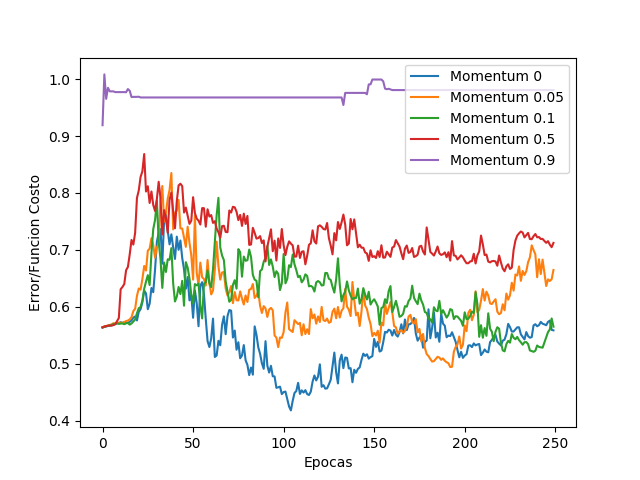
\includegraphics[width=1\linewidth]{graficos/eta_x_momentum_promedios_entrenamiento__2.png}
  \caption{Evolución del error de entrenamiento con momentum variable y learning rate fijo 0.1 (segunda vuelta)}
  \label{fig:sub2}
\end{subfigure}
\end{figure}

\begin{figure}[!htbp]
\centering
\begin{subfigure}{.5\textwidth}
  \centering
  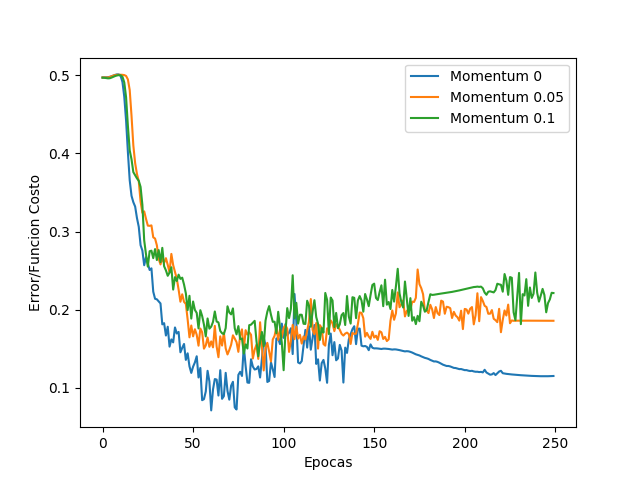
\includegraphics[width=1\linewidth]{graficos/eta_x_momentum_promedios_validacion__0.png}
  \caption{Evolución del error de validación con momentum variable y learning rate fijo 0.05 (segunda vuelta)}
  \label{fig:sub1}
\end{subfigure}%
\begin{subfigure}{.5\textwidth}
  \centering
  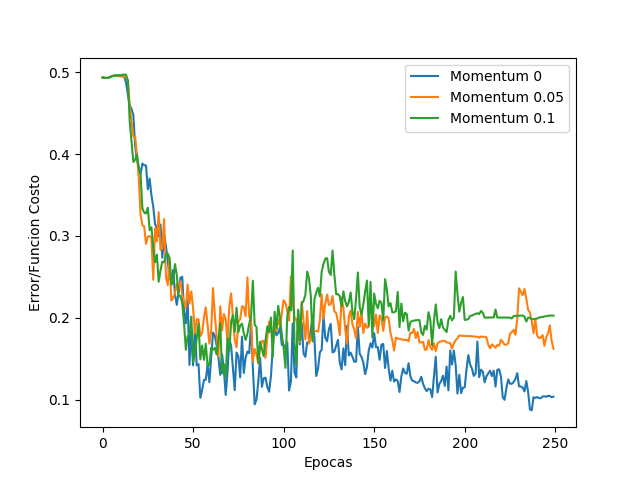
\includegraphics[width=1\linewidth]{graficos/eta_x_momentum_promedios_validacion__2.png}
  \caption{Evolución del error de validación con momentum variable y learning rate fijo 0.1 (segunda vuelta)}
  \label{fig:sub2}
\end{subfigure}
\end{figure}

Finalmente, confirmamos que, con estos resultados entre learning rate \textbf{0.1 y de 0.05}, la mejor opción es utilizar momentum \textbf{0}, como habíamos 
confirmado en experimentos anteriores, y learning rate (si bien no hay grandes diferencias en el error de validación obtenido) de \textbf{0.05} ya que 
registra el error más bajo tanto para entrenamiento como para validación.

\subsubsection{Performance de la red, variando simultáneamente técnicas de entrenamiento y de inicialización de pesos}

En este experimento decidimos también probar dos variables en simultáneo. Probamos la performance de las redes utilizando
distintas técnicas de entrenamiento: estocástico, batch y mini batch con distintos tamaños. Al mismo tiempo, variamos 
la distribución utilizada para la inicialización de los pesos de la red. Utilizamos distribución normal y uniforme.\\

A la hora de elegir tamaños de batch para las ejecuciones mini batch, elegimos los siguientes tamaños: 5,10,100, mitad del dataset y dataset completo (batch). La idea es probar con batchs pequeños como 5 y 10, 
cercanos al online learning y también con algunos tamaños más grandes. 
Probamos también utilizando el dataset completo.\\

Al igual que en los primeros dos experimentos, juzgaremos las modalidades midiendo la performance final de error sobre dataset de training, error sobre el de validación y efectividad de aciertos prediciendo los patrones de testing.\\
Observemos los resultados:

\begin{figure}[h]
  \begin{center}
  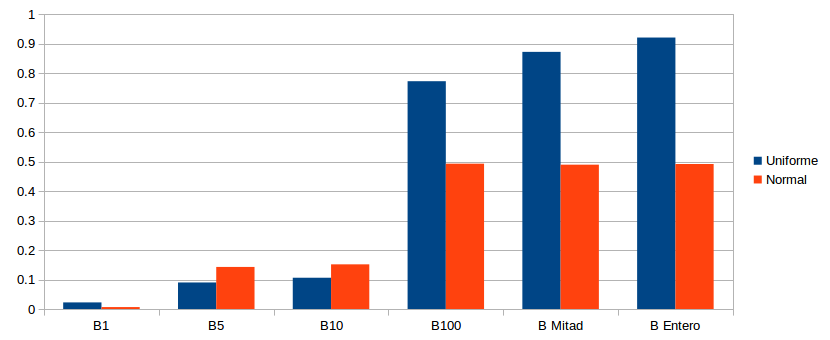
\includegraphics[scale=0.65]{graficos/distribucion_error_final.png}
  \caption{Error final (función de costo) promedio para cada cantidad de neuronas utilizando el dataset de entrenamiento}
  \end{center}
\end{figure}

En la primera figura de este experimento mostramos la función de costo obtenida con las diferentes técnicas.

Notación:
\begin{itemize}
\item $B1$ = Entrenamiento estocástico.
\item $BX$ = Mini batch de tamaño $X$.
\item $B$ $Mitad$ = Mini batch de tamaño equivalente a la mitad del dataset.
\item $B$ $Entero$ = Batch común.
\end{itemize}

A su vez, mostramos en color azul los resultados obtenidos utilizando distribución de pesos uniforme y en naranja, distribución normal.\\
Con respecto a los diferentes tipos de entrenamiento, notamos que el aprendizaje online obtiene mucho mejores resultados que las demás técnicas. El experimento muestra también que a medida que se utiliza un batch más grande, la precisión del modelo empeora. En algunos casos, muy notablemente.\\

Podemos ver además que,  para los mini batchs más pequeños, se obtuvieron mejores resultados utilizando la distribución uniforme. Sin embargo, tanto el aprendizaje estocástico como los batchs más grandes mostraron mejor rendimiento con la distribución normal. Es necesario aclarar que en el caso del entrenamiento estocástico la diferencia es muy pequeña y los resultados con ambas modalidades fueron muy parejos.\\

Para el error final en los datos de validación, obtuvimos los siguientes resultados:\\

\begin{figure}[h]
  \begin{center}
  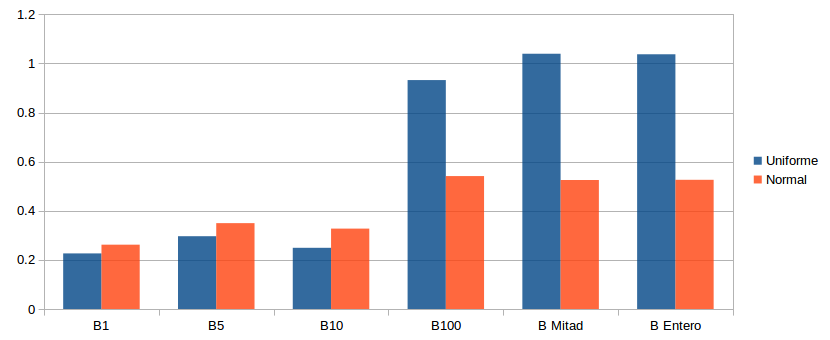
\includegraphics[scale=0.65]{graficos/distribucion_error_validacion.png}
  \caption{Error (función de costo) promedio para cada cantidad de neuronas utilizando el dataset de validación}
  \end{center}
\end{figure}

Aquí en la figura 24 se mantiene la misma tendencia que en los números anteriores. Los mejores resultados se obtuvieron con el online learning y con los mini batchs más pequeños.\\

En cuanto a los pesos iniciales, nuevamente observamos que la uniforme genera mejores resultados en los batchs más pequeños y la normal en los mayores.

\begin{figure}[h]
  \begin{center}
  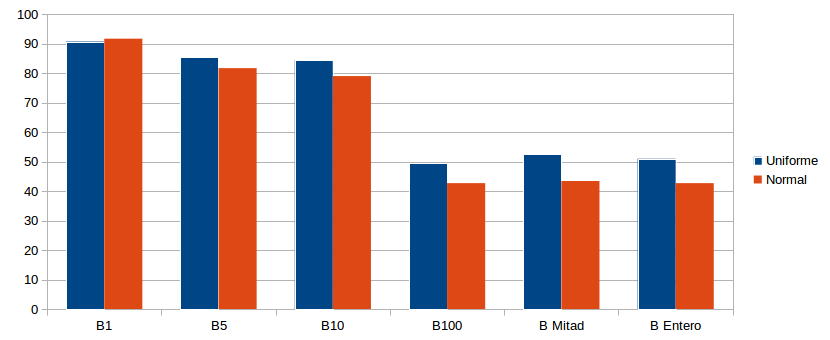
\includegraphics[scale=0.65]{graficos/distribucion_eficiencia.png}
  \caption{Tasa de predicciones correctas, en porcentaje, para el dataset de testing}
  \end{center}
\end{figure}

Por último la figura 25 muestra la tasa de aciertos sobre el dataset de testing. El mejor puntaje fue obtenido nuevamente por el entrenamientoe estocástico, con distribución normal. Estocástico con distribución uniforme también obtuvo buen número de aciertos, levemente menor que la normal.\\

Curiosamente todas las demás técnicas de entrenamiento muestran mejores predicciones con distribución uniforme. Esto contradice lo que había sucedido con las funciones de costo de los batchs B5 y B10 en las figuras 23 y 24. Sin embargo para B100, BM y BE, la uniforme nuevamente obtuvo los mejores resultados.\\

En vistas a los número registrados en el experimento, \textbf{resulta evidente que el entrenamiento estocástico tuvo mucho mejor rendimiento que todas las demás modalidades}. Particularmente los batchs mayores tuvieron una performance pobre, con altos valores de error y mala tasa de predicción.\\

En cuanto a distribución de pesos, el estocástico presentó menor error de entrenamiento y mejor tasa de predicción con distribución normal. La distribución uniforme tuvo un error levemente inferior para el dataset de validación. Los resultados en cuanto este factor fueron muy parejos.

\subsubsection{Performance de la red, sin y con preprocesamiento de los patrones.}

Una vez finalizado el desarrollo del perceptrón, comenzamos a probarlo con distintos datasets sencillos y pequeños encontrados en internet. En cuanto verificamos que estábamos obteniendo resultados coherentes, decidimos empezar a probar con los datos reales de los problemas del enunciado.\\

A esa altura, aún no teníamos listos los métodos de preprocesamiento de patrones. Lo que observamos fue que no nos era posible procesar los patrones del ejercicio 1 ya que al momento de aplicar varias de las operaciones matemáticas con los pesos y los inputs, se generaban errores de overflowing. Es decir, los valores con los que se estaba operando eran tan grandes que no permitía a la red almacenarlos en variables. Esto sucedió con los cálculos de las funciones de activación, usanto tando la logística como la tangente.\\

Decidimos entonces preprocesar los datos. Lo que realiza el programa es una normalización de los datos. Toma cada valor de cada atributo del problema y realiza 
la siguiente operación:\\

\begin{center}
	$valor_normalizado = (valor_original - media) / desvio$
\end{center}

Donde $media$ y $desvio$ son la media y el desvío estándar de todos los valores del atributo. De esta forma, se reducen los viejos valores a nuevos números más pequeños, centrados alrededor de la media.\\

Utilizamos este método a lo largo de todos los experimentos del trabajo. El resultado es que no podemos realizar pruebas sin normalizar los datos, ya que el programa genera errores de ejecución por overflow. Como consecuencia, no podemos experimentar en las diferencias de performance entre utilizar o no preprocesamiento de patrones ya que no utilizarlos nos impide ejecutar nuestro programa. Por ello, no presentamos experimentos con esta modalidad.

\subsubsection{Performance de la red, sin y con early-stopping.}

Early stopping es un método que nos permmite frenar el entrenamiento antes de que nuestra red sea afectada por el \textbf{overfitting}. Para implementarlo, 
luego de finalizada cada época del entrenamiento, si el error de validación esta por debajo del threshold (o valor del early stopping), entonces el 
entrenamiento termina sin necesidad de terminar de correr las épocas faltantes. De esta manera, la red no seguirá entrenando sobre el mismo conjunto de 
entrenamiento hasta que el error sea casi nulo, provocando así que al intentar predecir con nuevos datos, la red tenga una efectividad muy baja.

Para este experimento decidimos entrenar la red con diferentes valores del threshold, los cuales son \textbf{0, 0.2, 0.15, 0.1, 0.05 y 0.01}. La 
idea es poder determinar cual arroja mejores resultados sobre el conjunto de testing cuando se corta el entrenamiento para errores de validación por 
debajo de estos thresholds. Además, utilizamos entrenamientos de 500 épocas, para poder ver un poco mejor la diferencia entre tener y no tener 
early stopping.

\begin{figure}[!htbp]
\centering
\begin{subfigure}{.5\textwidth}
  \centering
  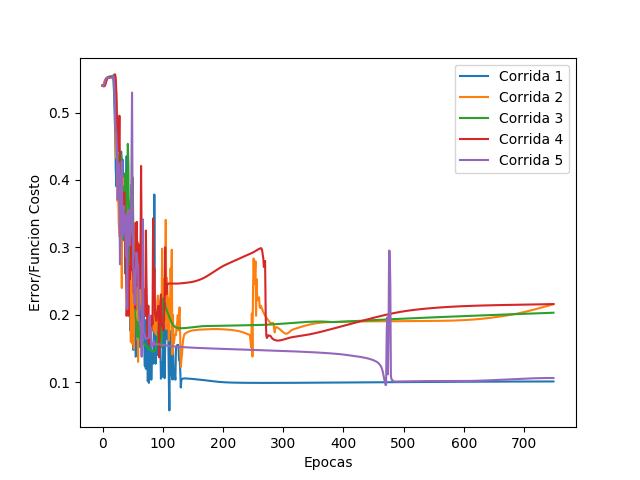
\includegraphics[width=1\linewidth]{graficos/early_stopping_validacion_0.png}
  \caption{Evolución del error de validación sin early stopping.}
  \label{fig:sub1}
\end{subfigure}%
\begin{subfigure}{.5\textwidth}
  \centering
  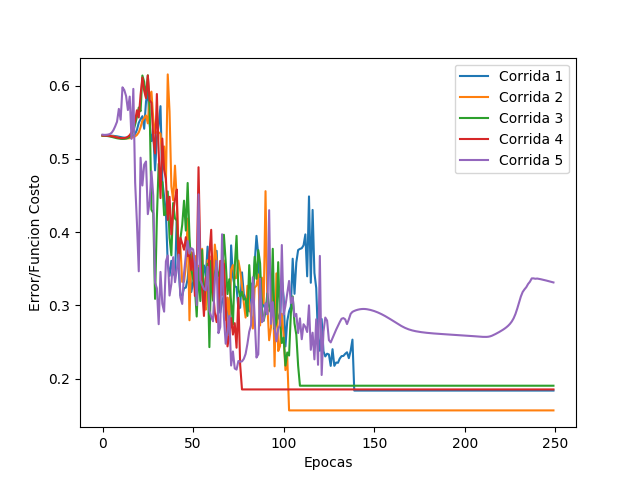
\includegraphics[width=1\linewidth]{graficos/early_stopping_validacion_0_2.png}
  \caption{Evolución del error de validación con early stopping. Threshold: 0.2}
  \label{fig:sub2}
\end{subfigure}
\end{figure}

\begin{figure}[!htbp]
\centering
\begin{subfigure}{.5\textwidth}
  \centering
  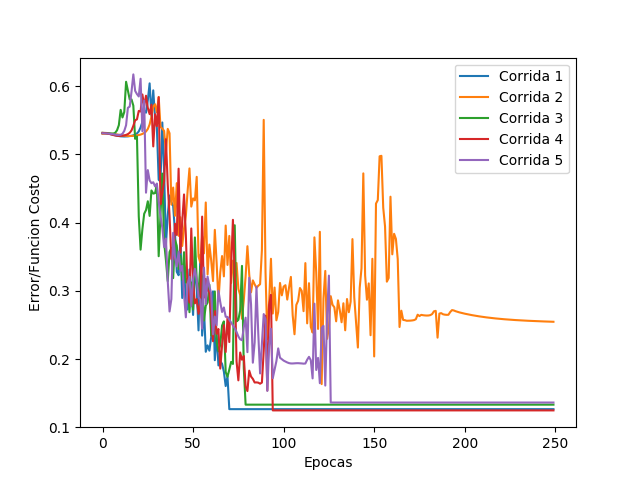
\includegraphics[width=1\linewidth]{graficos/early_stopping_validacion_0_15.png}
  \caption{Evolución del error de validación sin early stopping. Threshold: 0.15}
  \label{fig:sub1}
\end{subfigure}%
\begin{subfigure}{.5\textwidth}
  \centering
  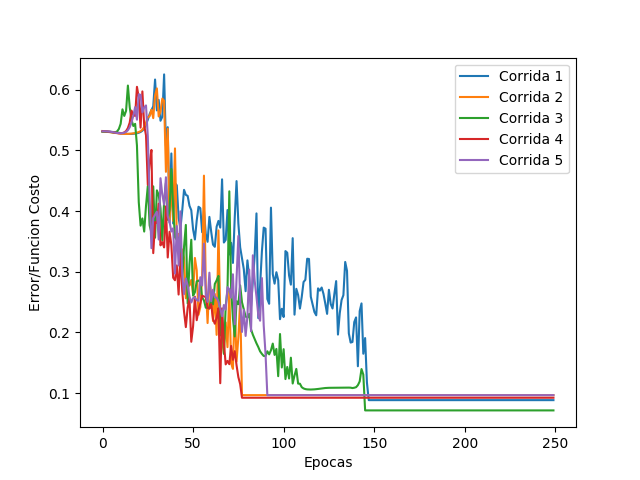
\includegraphics[width=1\linewidth]{graficos/early_stopping_validacion_0_1.png}
  \caption{Evolución del error de validación con early stopping. Threshold: 0.1}
  \label{fig:sub2}
\end{subfigure}
\end{figure}

\begin{figure}[!htbp]
\centering
\begin{subfigure}{.5\textwidth}
  \centering
  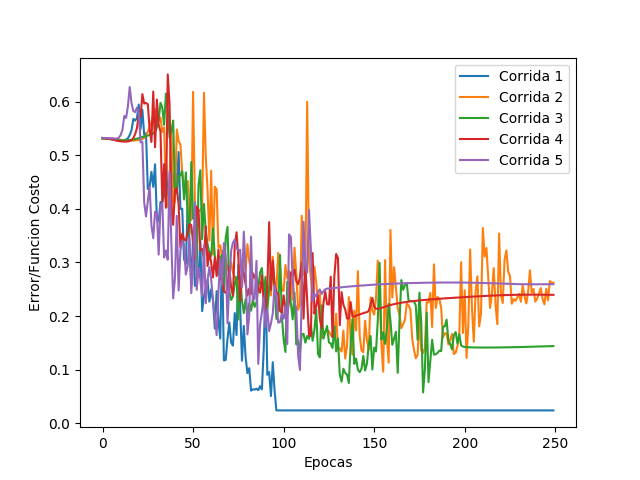
\includegraphics[width=1\linewidth]{graficos/early_stopping_validacion_0_05.png}
  \caption{Evolución del error de validación sin early stopping. Threshold: 0.05}
  \label{fig:sub1}
\end{subfigure}%
\begin{subfigure}{.5\textwidth}
  \centering
  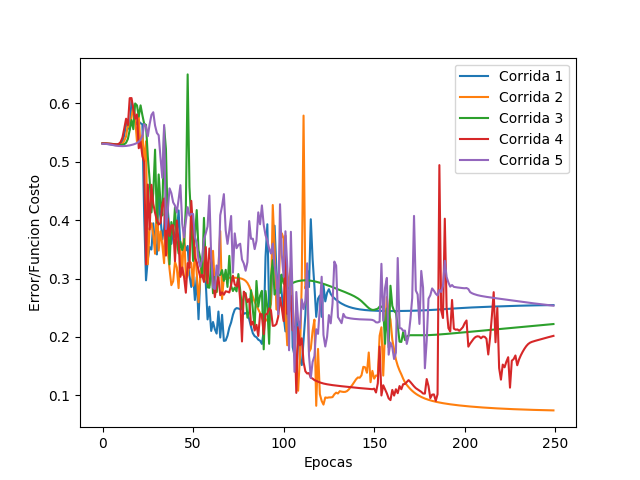
\includegraphics[width=1\linewidth]{graficos/early_stopping_validacion_0_01.png}
  \caption{Evolución del error de validación con early stopping. Threshold: 0.01}
  \label{fig:sub2}
\end{subfigure}
\end{figure}

\begin{figure}[!htbp]
  \begin{center}
  \includegraphics[scale=0.60]{graficos/early_stopping_testing_250ep.png}
  \caption{Resultados de eficiencia en la precisión al predecir los resultados del conjunto de datos de testing por threshold con 250 épocas}
  \end{center}
\end{figure}

Viendo los resultados, podemos aprecir que al no usar early stopping o usar un threshold de 0.01 se obtienen los mejores 
resultados sobre nuevos datos provenientes del conjunto de testing. Se puede ver además que usar un threshold muy bajo puede no ser alcanzado nunca por 
el conjunto de validación lo cual es lo mismo que entrenar la red sin early stopping, y esto es lo que sucedió al usar el threshold de 0.01. Contrario 
a esto, elegir un threshold muy alto produce que el entrenamiento termine rápidamente sin obtener una buena precisión para ningún tipo de dato, tanto 
los de entrenamiento y validación, como los de testing. Que no usar early stopping de los mejores resultados nos hace pensar que la cantidad de épocas 
durante las cuales corre nuestro entrenamiento no son lo suficientemente extensas como para provocar overfitting y saturar la red al punto que 
nueva información sea predecida erróneamente. 

Entendemos que, si bien en nuestro escenario el early stopping no mejoró nuestros resultados, en casos donde las épocas son muchas o las condiciones de 
la red provocan que si hay overfitting el error de validación comience a subir rápidamente, el early stopping puede hacer la diferencia en gran medidad. 
Para intentar simular esta situación, corrimos nuevamente las pruebas para 750 épocas, y los resultados apoyan esta idea: usar un threshold de \textbf{0.1} 
arrojo una eficiencia en \textbf{3\%} por encima de no usar early stopping.

\begin{figure}[!htbp]
  \begin{center}
  \includegraphics[scale=0.60]{graficos/early_stopping_testing_750ep.png}
  \caption{Resultados de eficiencia en la precisión al predecir los resultados del conjunto de datos de testing por threshold con 750 épocas}
  \end{center}
\end{figure}

Sabiendo esto, es importante a su vez saber seleccionar el threshold de early stopping entendiendo el conjunto de datos y analizando como evoluciona la 
red utilizada durante el entrenamiento, para evitar caer en los 2 casos antes mencionados. 

\subsubsection{Performance de la red, variando las funciones de activación y/o sus parámetros.}

\newpage
\subsection{Ejercicio 2}

Repetimos los experimentos para el ejercicio 2 para intentar obtener la mejor arquitectura para la solución de este problema.

\subsubsection{Variación del número de capas ocultas.}
La idea de este experimento, al igual que en el ejercicio 1, es determinar la cantidad de capas ocultas óptimas para la solución. Fijamos todas las variables con los mismos valores que para el experimento análogo del ejercicio 1.\\
Esta configuración es arbitraria y su propósito es únicamente setear valores fijos para experimentar con la cantidad de capas ocultas.\\

La modalidad del experimento fue la misma, probamos la performance de la red con 1, 2, 3 y 5 capas. No utilizamos valores mayores ya que fueron filtrados previamente debido a sus muy inferiores resultados.\\

Observemos los resultados de los distintos valores seleccionados:\\

\begin{figure}[h]
  \begin{center}
  \includegraphics[scale=0.75]{graficos/ej2_cant_capas_error_final.png}
  \caption{Error final (función de costo) promedio para cada cantidad de neuronas utilizando el dataset de entrenamiento}
  \end{center}
\end{figure}

Podemos ver aquí que todas las modalidades obtuvieron un error final bastante similar, prácticamente igual. Nos sorprendió la similitud de los resultados ya que no esperábamos tan pequeña diferencia.\\
Sabíamos previamente por consultas en clase que era probable que los valores más bajos de capas fueran los más óptimos para el problema, pero nuestros resultados muestran que subiendo incluso hasta 5 capas, el error final empeora pero muy sensiblemente.

Para el error final en los datos de validación, obtuvimos los siguientes resultados:\\

\begin{figure}[h]
  \begin{center}
  \includegraphics[scale=0.75]{graficos/ej2_cant_capas_error_valid.png}
  \caption{Error (función de costo) promedio para cada cantidad de neuronas utilizando el dataset de validación}
  \end{center}
\end{figure}

\newpage

Aquí se repite la tendencia, valores muy cercanos para todas las configuraciones.\\

Analicemos la tasa de aciertos sobre el dataset de testing.

\begin{figure}[h]
  \begin{center}
  \includegraphics[scale=0.75]{graficos/ej2_cant_capas_testing.png}
  \caption{Tasa de predicciones correctas, en porcentaje, para el dataset de testing}
  \end{center}
\end{figure}

Antes de explicar los números, aclaremos que para calcular la tasa de aciertos se utilizó el siguiente criterio. Primero, como este es un problema con 2 salidas, para considerar un patrón como bien predicho consideramos que ambos valores de salida debían estar cercanos a los valores esperados. La definición de \lq cercano \rq corresponde a estar a una distancia de al menos $0,25$ con el valor esperado. Este criterio es para poder salvar las pequeñas diferencias que surgen en el cálculo de cada salida. Al ser valores flotantes, no se obtienen coincidencias perfectas, sino aproximaciones.\\

Lo que nos interesaba es poder medir la cantidad de aciertos, con algún margen de error de tolerancia.\\

Podemos ver en los números que la arquitectura de 1 capa obtuvo mejores resultados que las demás, aunque no muy superiores. Es destacable que los porcentajes de aciertos son mucho menores que los del mismo experimento del ejercicio 1. Atribuimos esto al criterio antes explicado de cálculo de aciertos. Modificando el criterio de tolerancia se podrían obtener valores mayores, pero no es realmente lo que nos interesaba. Además en este problema se deben predecir 2 valores de salida distintos y se considera un acierto sólo si ambos están en el rango de tolerancia, por ende el criterio es más exigente.\\

Teniendo en cuenta los resultados presentados en estas pruebas, \textbf{nos decidimos por una arquitectura de 1 capa oculta como parte de la solución óptima.} Aunque se obtuvieron resultados casi igual de buenos con arquitecturas de 2 y 3 capas, notando una leve desmejora a medida que se subió la cantidad utilizada.

\subsubsection{Variación del número de neuronas ocultas.}

Este experimento es análogo al del número de neuronas ocultas del experimento 1. 
Elegimos las siguientes medidas: 1 capa de 2, 5, 7, 10, 15 y 20 neuronas. 

Para el error final, obtuvimos los siguientes resultados:\\

\begin{figure}[h]
  \begin{center}
  \includegraphics[scale=0.70]{graficos/ej2_cant_neuro_error_final.png}
  \caption{Error final (función de costo) promedio para cada cantidad de neuronas utilizando el dataset de entrenamiento}
  \end{center}
\end{figure}

En la figura anterior se puede observar que todas las configuraciones obtuvieron valores de función de costo en el rango de $0,8$ - $0,12$ notando una muy leve mejora para las capas de 5 y 7 neuronas. Al igual que en el experimento anterior, resulta llamativa la similitud de los resultados. \\

Para el error final en los datos de validación, obtuvimos los siguientes resultados:\\

\begin{figure}[h]
  \begin{center}
  \includegraphics[scale=0.70]{graficos/ej2_cant_neuro_error_valid.png}
  \caption{Error (función de costo) promedio para cada cantidad de neuronas utilizando el dataset de validación}
  \end{center}
\end{figure}

\newpage

Se mantiene la tendencia para el dataset de validación. Levemente mejores resultados para la arquitectura de 7 neuronas por capa.

Para la efectividad en la predicción de los datos de testing, obtuvimos:\\

\begin{figure}[h]
  \begin{center}
  \includegraphics[scale=0.70]{graficos/ej2_cant_neuro_testing.png}
  \caption{Tasa de predicciones correctas, en porcentaje, para el dataset de testing}
  \end{center}
\end{figure}

La tasa de aciertos se calculó con el método explicado en el experimento anterior. Notamos que la arquitectura de 2 neuronas obtuvo un resultado inferior a las demás. En cuanto a éstas, se destaca la de 5 y 7 neuronas con un porcentaje muy levemente mayor. Es curioso que, sacando el primer caso, todas hayan obtenido números tan similares. No logramos explicar con claridad el motivo de esta similitud.\\

Observando los resultados obtenidos en las pruebas, \textbf{decidimos que la configuración a utilizar es es 1 capa con 7 neuronas}. Podríamos haber elegido también la de 5 neuronas, ya que los resultados son prácticamente idénticos, con una leve ventaja para la arquitectura de 7.\\

\subsubsection{Performance de la red, variando simultáneamente técnicas de entrenamiento y de inicialización de pesos}

Este experimento es análogo al realizado para el ejercicio 1. Probamos la performance de las redes utilizando
distintas técnicas de entrenamiento: estocástico, batch y mini batch con distintos tamaños. Al mismo tiempo, variamos 
la distribución utilizada para la inicialización de los pesos de la red. Utilizamos distribución normal y uniforme.\\

Utilizamos los mismos valores de batch que en el ejercicio 1 y las mismas distribuciones, normal y uniforme.\\
Observemos los resultados:

\begin{figure}[h]
  \begin{center}
  \includegraphics[scale=0.65]{graficos/ej2_distribucion_error_final.png}
  \caption{Error final (función de costo) promedio para cada cantidad de neuronas utilizando el dataset de entrenamiento}
  \end{center}
\end{figure}

En la primera figura de este experimento mostramos la función de costo obtenida con las diferentes técnicas.\\

Al igual que en el problema del ejercicio 1, el aprendizaje estocástico obtuvo mejores resultados que los demás métodos, aunque de forma menos marcada. Nuevamente se observa también que los batchs más pequeños generan errores menores. \\

Notamos que para este ejercicio, las modalidades de batch y mini batch mostraron mucho mejor rendimiento que para el ejercicio 1. En aquel, estas modalidades, especialmente las de batchs grandes, generaban un error muy alto y resultados pobres.\\

Con respecto a las diferentes técnicas de inicialización, notamos que en todas las modalidades de entrenamiento, se observan resultados similares entre utilizar distribución normal y uniforme. Otra diferencia con los resultados del ejercicio 1, es que aquí no se notó tanta diferencia entre las distribuciones.\\

Para el error final en los datos de validación, obtuvimos los siguientes resultados:\\

\begin{figure}[h]
  \begin{center}
  \includegraphics[scale=0.65]{graficos/ej2_distribucion_error_validacion.png}
  \caption{Error (función de costo) promedio para cada cantidad de neuronas utilizando el dataset de validación}
  \end{center}
\end{figure}

En la prueba de validación obtuvimos resultados en la misma sintonía. Ventaja en rendimiento del aprendizaje online y números parejos para la comparación entre distribuciones.

\begin{figure}[h]
  \begin{center}
  \includegraphics[scale=0.65]{graficos/ej2_distribucion_eficiencia.png}
  \caption{Tasa de predicciones correctas, en porcentaje, para el dataset de testing}
  \end{center}
\end{figure}

En los resultados de testing observamos la misma tendencia. Mejores resultados del aprendimiento online, con la curiosidad que aquí, a diferencia del ejercicio 1, la distribución uniforme presenta una leve ventaja.\\
En todos los demás casos, predomina la normal. Nuevamente esto resultó contrario a lo analizado en este mismo experimento para el ejercicio 1.\\

Para todos los tamaños de batch, se mantuvo fijo la relación de efectividad entre cada una de las distribuciones.\\

Teniendo en cuenta los resultados obtenidos, podemos concluir que \textbf{el entrenamiento estocástico tuvo levemente mejor rendimiento que las demás modalidades}. Los resultados no son tan contundentes como en el ejercicio 1.\\

En cuanto a distribución de pesos, el aprendizaje estocástico presentó una muy leve ventaja en resultados utilizando distribución uniforme. La diferencia es mínima, al igual que en el problema 1. Sospechamos que la elección de distrubición de pesos no afecta muy significativamente los resultados finales de la red, al menos en estos casos analizados.\\

\subsubsection{Performance de la red, variando simultáneamente el factor de aprendizaje $\mu$, y el parámetro $\alpha$ del momentum.}

Para el ejercicio 2 decidimos, en vez de hacer pruebas con y sin momentum por un lado, y variar el eta y el momentum por otro, de hacerlo todo junto.
El experimento es similar que en el ej1 pero tomamos los siguiente valores de momentum: \textbf{0, 0.05, 0.1, 0.5 y 0.9}, los cuales se 
probaron con los valores de learning rate \textbf{0.05, 0.08, 0.1, 0.12, 0.15 y 0.2}. Vamos a mostrar solo los resultados sobre el error de validación 
en conjunto con el error de testing, que son los datos que definen que tan bien está preparada la red para predecir nuevos datos.

\begin{figure}[!htbp]
\centering
\begin{subfigure}{.5\textwidth}
  \centering
  \includegraphics[width=1\linewidth]{graficos/ej2/eta_x_momentum_promedios_validacion_0_05.png}
  \caption{Evolución del error de validación con momentum variable y learning rate fijo 0.05}
  \label{fig:sub1}
\end{subfigure}%
\begin{subfigure}{.5\textwidth}
  \centering
  \includegraphics[width=1\linewidth]{graficos/ej2/eta_x_momentum_promedios_validacion_0_08.png}
  \caption{Evolución del error de validación con momentum variable y learning rate fijo 0.08}
  \label{fig:sub2}
\end{subfigure}
\end{figure}

\begin{figure}[!htbp]
\centering
\begin{subfigure}{.5\textwidth}
  \centering
  \includegraphics[width=1\linewidth]{graficos/ej2/eta_x_momentum_promedios_validacion_0_1.png}
  \caption{Evolución del error de validación con momentum variable y learning rate fijo 0.1}
  \label{fig:sub1}
\end{subfigure}%
\begin{subfigure}{.5\textwidth}
  \centering
  \includegraphics[width=1\linewidth]{graficos/ej2/eta_x_momentum_promedios_validacion_0_12.png}
  \caption{Evolución del error de validación con momentum variable y learning rate fijo 0.12}
  \label{fig:sub2}
\end{subfigure}
\end{figure}

\begin{figure}[!htbp]
\centering
\begin{subfigure}{.5\textwidth}
  \centering
  \includegraphics[width=1\linewidth]{graficos/ej2/eta_x_momentum_promedios_validacion_0_15.png}
  \caption{Evolución del error de validación con momentum variable y learning rate fijo 0.15}
  \label{fig:sub1}
\end{subfigure}%
\begin{subfigure}{.5\textwidth}
  \centering
  \includegraphics[width=1\linewidth]{graficos/ej2/eta_x_momentum_promedios_validacion_0_2.png}
  \caption{Evolución del error de validación con momentum variable y learning rate fijo 0.2}
  \label{fig:sub2}
\end{subfigure}
\end{figure}


A partir de los resultados podemos apreciar que los valores más bajos del error de validación se obtuvieron con learning rate \textbf{0.05}. Dado esto,
decidimos hacer unas pruebas extras con learning rates de \textbf{0.01 y 0.03} pero no conseguimos mejores resultados. 

\begin{figure}[!htbp]
  \begin{center}
  \includegraphics[scale=1]{graficos/ej2/error_testing_eta_x_momentum.png}
  \caption{Tasa de predicciones correctas, en porcentaje, para el dataset de testing}
  \end{center}
\end{figure}

Analizando también los datos de eficiencia sobre el conjunto de testing, podemos ver que la combinación de momentum 0 y learning rate 0.05 es la que 
mejor resultados da, y será nuestra elección. Sin embargo, es importante notar que muy buenos resultados se pueden lograr también con learnig rate 
0.1 y momentum 0, y con learning rate 0.12 y momentum 0.05.


\subsection{Descripción, justificación y performance, de la solución óptima propuesta.}


\subsection{Conclusiones.}

	\newpage
	\section{Apéndice - Código}

	\newpage
	\section{Bibliografía}
	\label{marker}

\begin{thebibliography}{9}

\bibitem{jefflee}
ANSI C Yacc grammar - Jeff Lee\\
 \url{https://www.lysator.liu.se/c/ANSI-C-grammar-y.html}

\end{thebibliography}
\end{document}

